\chapter{Системийн дэлгэрэнгүй материал}

Энэхүү хавсралтад 4-р бүлгийн үндсэн тайлбарыг дэмжих дэлгэрэнгүй хүснэгт, хэрэглээний тохиолдлын нарийвчилсан зураг, системийн урсгалын нэмэлт диаграммуудыг нэгтгэн оруулав.

\section{Функциональ шаардлагын дэлгэрэнгүй хүснэгт}

{\footnotesize
\setlength{\tabcolsep}{3pt}
\captionof{table}{Системийн функциональ шаардлагууд I}\label{app:functional-1}
\begin{longtable}{|L{1.3cm}|L{2.5cm}|L{5.4cm}|L{4.0cm}|}
\hline
\textbf{Код} & \textbf{Модуль} & \textbf{Функциональ шаардлага} & \textbf{Баталгаажуулах шалгуур} \\
\hline
\endfirsthead
\hline
\textbf{Код} & \textbf{Модуль} & \textbf{Функциональ шаардлага} & \textbf{Баталгаажуулах шалгуур} \\
\hline
\endhead
ФШ-01 & Бүртгэл ба хандалт & Систем нь хэрэглэгчийг бүртгэх, нэвтрүүлэх, зөвшөөрөгдсөн өгөгдөлдөө хандах боломж олгоно. & Хэрэглэгч амжилттай бүртгүүлж, нэвтэрч, өөрийн өгөгдлийг бусдын өгөгдлөөс тусгаарлан харах боломжтой байна. \\
\hline
ФШ-02 & Дадлын удирдлага & Систем нь дадал үүсгэх, засах, архивлах боломжтой байна. & Үүсгэсэн, зассан, архивласан дадлын төлөв өгөгдлийн санд зөв хадгалагдаж, дахин нээхэд зөв харагдана. \\
\hline
ФШ-03 & Хуваарь & Систем нь дадлын давтамж, идэвхтэй өдрүүд, хэрэгжих хугацааны хүрээг тохируулах боломжтой байна. & Хэрэглэгчийн сонгосон хуваарь зөв хадгалагдаж, тухайн өдрүүдэд зөв идэвхжинэ. \\
\hline
ФШ-04 & Хэмжилт & Систем нь дадлыг тоо, удаа, хугацаа зэрэг хэмжилтийн төрлөөр бүртгэх боломжтой байна. & Сонгосон хэмжилтийн төрөлд тохирсон оролт хүлээн авч, гүйцэтгэлийн утгыг зөв хадгална. \\
\hline
ФШ-05 & Сэдлийн профайл & Систем нь дадал бүрт зорилгын шошго, хувийн шалтгаан, өөрийн дүр төрхийн тодорхойлолтыг хадгална. & Оруулсан сэдлийн мэдээлэл зөв хадгалагдаж, дараа дахин нээхэд зөв дуудагдана. \\
\hline
ФШ-06 & Өдөөгч нөхцөл & Систем нь дадал бүрт өдрийн цаг, ерөнхий байршил, өмнөх үйлдэл зэрэг өдөөгч нөхцөл тохируулах боломжтой байна. & Тохируулсан өдөөгч нөхцөлүүд зөв хадгалагдаж, сануулгын шийдвэрийн логикт ашиглагдана. \\
\hline
ФШ-07 & Сануулга & Систем нь хуваарь болон өдөөгч нөхцөлд тулгуурлан нөхцөл байдалд нийцсэн сануулга үүсгэж, илгээнэ. & Сануулга үүссэн тохиолдол бүр бүртгэлтэй байх бөгөөд ижил нөхцөлд давхардсан илгээлт үүсэхгүй байна. \\
\hline
ФШ-08 & Сануулгын тайлбар & Систем нь сануулга тухайн мөчид яагаад илгээгдсэнийг тайлбарлан харуулна. & Сануулгын дэлгэрэнгүй мэдээлэл дотор шийдвэрт нөлөөлсөн үндсэн нөхцөлүүдийг харуулах боломжтой байна. \\
\hline
ФШ-09 & Сануулгын үйлдэл & Систем нь сануулгад өгсөн хэрэглэгчийн үйлдлийг бүртгэнэ. & ``Хийлээ'', ``дараа сануул'' зэрэг үйлдлийн сонголт бүр лог хэлбэрээр хадгалагдана. \\
\hline
ФШ-10 & Хурдан бүртгэл & Систем нь дадлын гүйцэтгэлийг цөөн алхмаар бүртгэх боломжтой байна. & Үндсэн гүйцэтгэл бүртгэх урсгал нь гол дэлгэцээс шууд эхэлж, илүүц шат дамжлагагүй байна. \\
\hline
ФШ-11 & Гүйцэтгэлийн бүртгэл & Систем нь дадлын гүйцэтгэлийг ``хийсэн'', ``хэсэгчлэн хийсэн'', ``хийгээгүй'' төлвөөр бүртгэнэ. & Гүйцэтгэлийн төлөв, тоон утга, бүртгэсэн хугацаа зөв хадгалагдана. \\
\hline
ФШ-12 & Жижиг алхам & Систем нь дадлыг жижиг алхмуудад хувааж, алхам тус бүрийн явцыг бүртгэх боломжтой байна. & Нэг дадалд олон жижиг алхам холбогдож, алхам тус бүрийн төлөв тусад нь хадгалагдана. \\
\hline
ФШ-13 & Урьдчилсан төлөвлөгөө & Систем нь ``хэрэв--тэгвэл'' хэлбэрийн урьдчилсан төлөвлөгөө үүсгэх боломжтой байна. & Хэрэглэгч нөхцөл ба түүнд хариу үйлдэл гэсэн хоёр хэсэгтэй төлөвлөгөө үүсгэж, хадгалах боломжтой байна. \\
\hline
\end{longtable}
}

{\footnotesize
\setlength{\tabcolsep}{3pt}
\captionof{table}{Системийн функциональ шаардлагууд II}\label{app:functional-2}
\begin{longtable}{|L{1.3cm}|L{2.5cm}|L{5.4cm}|L{4.0cm}|}
\hline
\textbf{Код} & \textbf{Модуль} & \textbf{Функциональ шаардлага} & \textbf{Баталгаажуулах шалгуур} \\
\hline
\endfirsthead
\hline
\textbf{Код} & \textbf{Модуль} & \textbf{Функциональ шаардлага} & \textbf{Баталгаажуулах шалгуур} \\
\hline
\endhead
ФШ-14 & Хэцүү байдлын үнэлгээ & Систем нь дадлыг гүйцэтгэхэд хэр хэцүү байсныг хэрэглэгчээс үнэлгээ хэлбэрээр авна. & Гүйцэтгэлийн дараа хэцүү байдлын үнэлгээ авах, хадгалах, холбогдох дадалтай уялдуулах боломжтой байна. \\
\hline
ФШ-15 & Дасан зохицох санал & Систем нь сул гүйцэтгэл, өндөр төвөгшил, тогтворгүй ахицын үед дадлыг хялбаршуулах эсвэл нөхцөлийг өөрчлөх санал гаргана. & Санал үүсэх нөхцөл тодорхой дүрэмтэй байх бөгөөд үүссэн санал нь тайлбартай хадгалагдана. \\
\hline
ФШ-16 & Гүйцэтгэлийн эх үүсвэр & Систем нь гүйцэтгэлийг сануулгад тулгуурласан, өөрийн санаачилгатай, тодорхойгүй гэж ангилан хадгална. & Гүйцэтгэлийн бүртгэл бүр дээр эх үүсвэрийн ангилал хадгалагдана. \\
\hline
ФШ-17 & Тасралтгүй цуваа & Систем нь дараалсан гүйцэтгэлийг тооцоолж, тасралт үүссэн эсэхийг бүртгэнэ. & Гүйцэтгэлийн түүх өөрчлөгдөхөд цувааны урт дахин тооцоологдож, тасралтын төлөв зөв шинэчлэгдэнэ. \\
\hline
ФШ-18 & Богино урамшуулал & Систем нь гүйцэтгэлийн дараа богино урамшууллын буцаан холбоо үзүүлнэ. & Амжилттай гүйцэтгэлийн дараа баяр хүргэлт, оноо эсвэл тэмдэг зэрэг урамшууллын үйл явдал үүснэ. \\
\hline
ФШ-19 & Эргэцүүлсэн санал сэтгэгдэл & Систем нь гүйцэтгэлийн дараах ашиг тусын эргэцүүллийг авах боломжтой байна. & Хэрэглэгч эрч хүч, төвлөрөл, сэтгэл санаа зэрэг товч эргэцүүллийг бөглөж хадгалах боломжтой байна. \\
\hline
ФШ-20 & Автоматжилтын үнэлгээ & Систем нь зан үйлийн автоматжсан байдлын өөрөө тайлагнах индекс (SRBAI)-д суурилсан үнэлгээг тодорхой давтамжаар авч хадгална. & Асуулгын хариулт бүр хугацааны тэмдэгтэй хадгалагдаж, оноо автоматаар тооцоологдоно. \\
\hline
ФШ-21 & Дадлын хүчний оноо & Систем нь автоматжилтын үнэлгээ болон зан үйлийн прокси үзүүлэлтэд тулгуурлан дадлын хүчний оноо тооцоолно. & Оноо тооцоход оролцсон үзүүлэлтүүд болон эцсийн үр дүн бүртгэлтэй хадгалагдана. \\
\hline
ФШ-22 & Сануулгыг аажмаар бууруулах & Систем нь дадал бэхжихийн хэрээр сануулгын эрчмийг аажмаар бууруулна. & Бэхжилтийн түвшин өсөхөд сануулгын бодлого шинэчлэгдэж, өөрчлөлт нь бүртгэлтэй хадгалагдана. \\
\hline
ФШ-23 & Ахицын шинжилгээ & Систем нь ахиц, цуваа, гүйцэтгэлийн түүх, бэхжилтийн өөрчлөлтийг ойлгомжтой хэлбэрээр харуулна. & Хяналтын самбарт шаардлагатай үндсэн үзүүлэлтүүд зөв тооцоологдон харагдана. \\
\hline
ФШ-24 & Хуваалцах & Систем нь урамшуулал, цуваа, ахицын мэдээллийг хуваалцах боломж олгоно. & Сонгосон ахицын мэдээллээр хуваалцах зураг эсвэл карт үүсгэх боломжтой байна. \\
\hline
ФШ-25 & Шинжилгээний өгөгдөл & Систем нь хэрэглээний болон зан үйлийн шинжилгээнд шаардлагатай өгөгдлийг бүртгэнэ. & Судалгаанд шаардлагатай үйл явдлын өгөгдөл хугацааны тэмдэг, эх үүсвэр, холбогдох өгөгдөлтэй хадгалагдана. \\
\hline
\end{longtable}
}

\section{Функциональ бус шаардлагын дэлгэрэнгүй хүснэгт}

\begin{table}[htbp]
\centering
\footnotesize
\setlength{\tabcolsep}{3pt}
\begin{tabular}{|L{1.4cm}|L{2.2cm}|L{5.7cm}|L{4.1cm}|}
\hline
\textbf{Код} & \textbf{Ангилал} & \textbf{Функциональ бус шаардлага} & \textbf{Хэмжигдэх шалгуур} \\
\hline
ФБШ-01 & Ашиглахад хялбар байдал & Үндсэн хэрэглээний урсгалууд ойлгомжтой, цөөн алхамтай байх ёстой. & Сануулгаас гүйцэтгэл бүртгэх үйлдэл 1 товшилтоор, үндсэн дэлгэцээс 2-оос ихгүй алхмаар хийгдэх \\
\hline
ФБШ-02 & Гүйцэтгэл & Гол дэлгэцүүд болон чухал үйлдлүүд богино хугацаанд хариу өгөх ёстой. & Гол дэлгэц ачаалах хугацаа 2 секундээс ихгүй, гүйцэтгэл хадгалах хугацаа 1 секундээс ихгүй \\
\hline
ФБШ-03 & Найдвартай байдал & Гүйцэтгэлийн бүртгэл, сануулгын үйлдэл, урамшууллын мэдээлэл, автоматжилтын үнэлгээ алдагдалгүй хадгалагдах ёстой. & Туршилтын өгөгдлийн бүрэн бүтэн байдал 100 хувь байх \\
\hline
ФБШ-04 & Аюулгүй байдал & Хэрэглэгчийн өгөгдлийг зөвшөөрөлгүй хандалтаас хамгаалах ёстой. & Нууц үгийг хэш хэлбэрээр хадгалах, баталгаажсан хандалт шаардах \\
\hline
ФБШ-05 & Нууцлал & Систем зөвхөн шаардлагатай хамгийн бага нөхцөл байдлын мэдээллийг ашиглах ёстой. & Байршлын өгөгдөл ерөнхий ангиллын түвшинд хадгалагдах \\
\hline
ФБШ-06 & Тохирох чадвар & Систем түгээмэл орчин үеийн хөтөч болон хөдөлгөөнт орчинд ажиллах ёстой. & Chrome, Edge, Safari дээр үндсэн урсгалууд алдаагүй ажиллах \\
\hline
ФБШ-07 & Засварлах ба өргөтгөх чадвар & Системийн бүтэц нь модульчилсан, өргөтгөх, засварлахад хялбар байх ёстой. & Интерфэйс, хэрэглээний логик, домайн логик, өгөгдлийн түвшин тусгаарлагдсан байх \\
\hline
ФБШ-08 & Ачаалал даах чадвар & Туршилтын түвшинд өгөгдлийн хэмжээ өсөхөд үндсэн ажиллагаа тогтвортой байх ёстой. & Олон дадал, олон бүртгэлтэй өгөгдөл дээр ажиллагаа хэвийн үргэлжлэх \\
\hline
ФБШ-09 & Ажиглагдах чадвар & Судалгааны үзүүлэлтүүдийг тооцоход хангалттай аналитик өгөгдөл бүртгэгдэх ёстой. & Хэрэглээний болон зан үйлийн үзүүлэлтүүдийг тооцох боломжтой байх \\
\hline
ФБШ-10 & Алдаа зохицуулалт & Алдаа гарсан үед систем ойлгомжтой мэдээлэл өгч, өгөгдлийг буруу төлөвт оруулахгүй байх ёстой. & Алдааны мэдээлэл, дахин оролдох логик ажиллах \\
\hline
\end{tabular}
\caption{Системийн функциональ бус шаардлагууд}
\end{table}

\section{Хэрэглээний тохиолдол ба системийн урсгалын нэмэлт диаграммууд}

\begin{figure}[H]
    \centering
    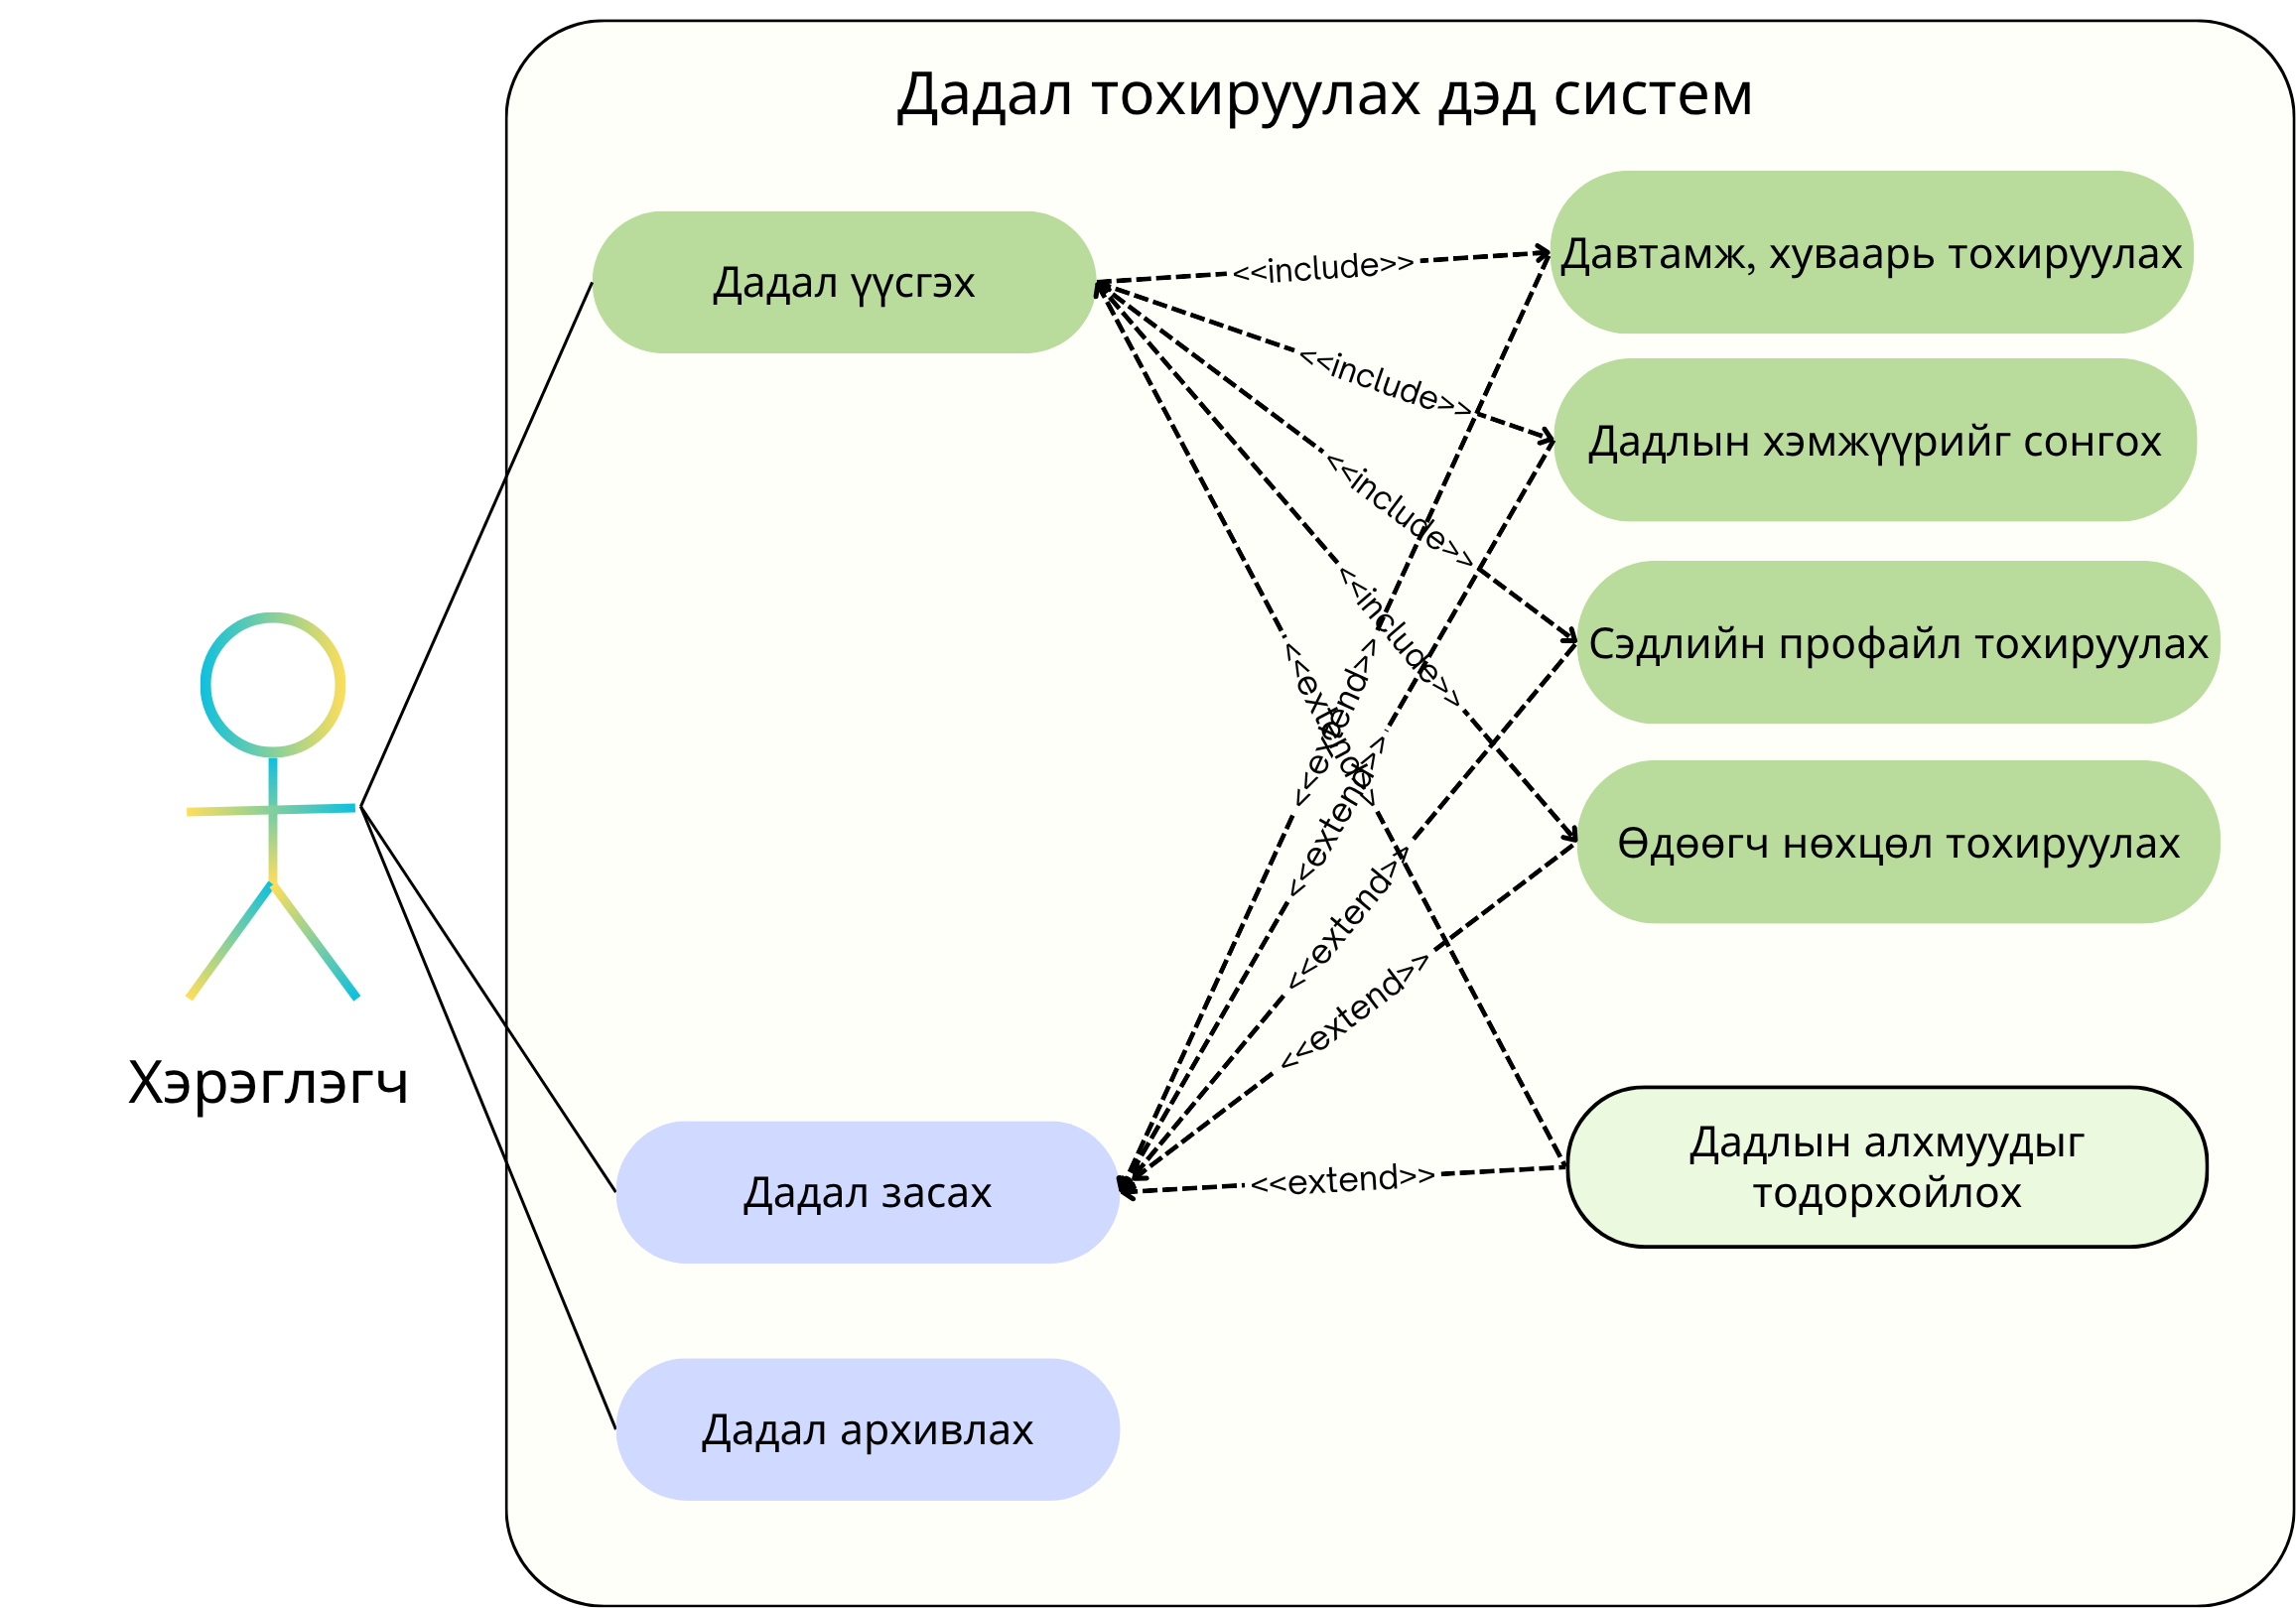
\includegraphics[width=0.84\textwidth]{images/HabitManagementUseCase.png}
    \caption{Дадал үүсгэх ба удирдах хэрэглээний тохиолдлын диаграмм}
\end{figure}

\begin{figure}[H]
    \centering
    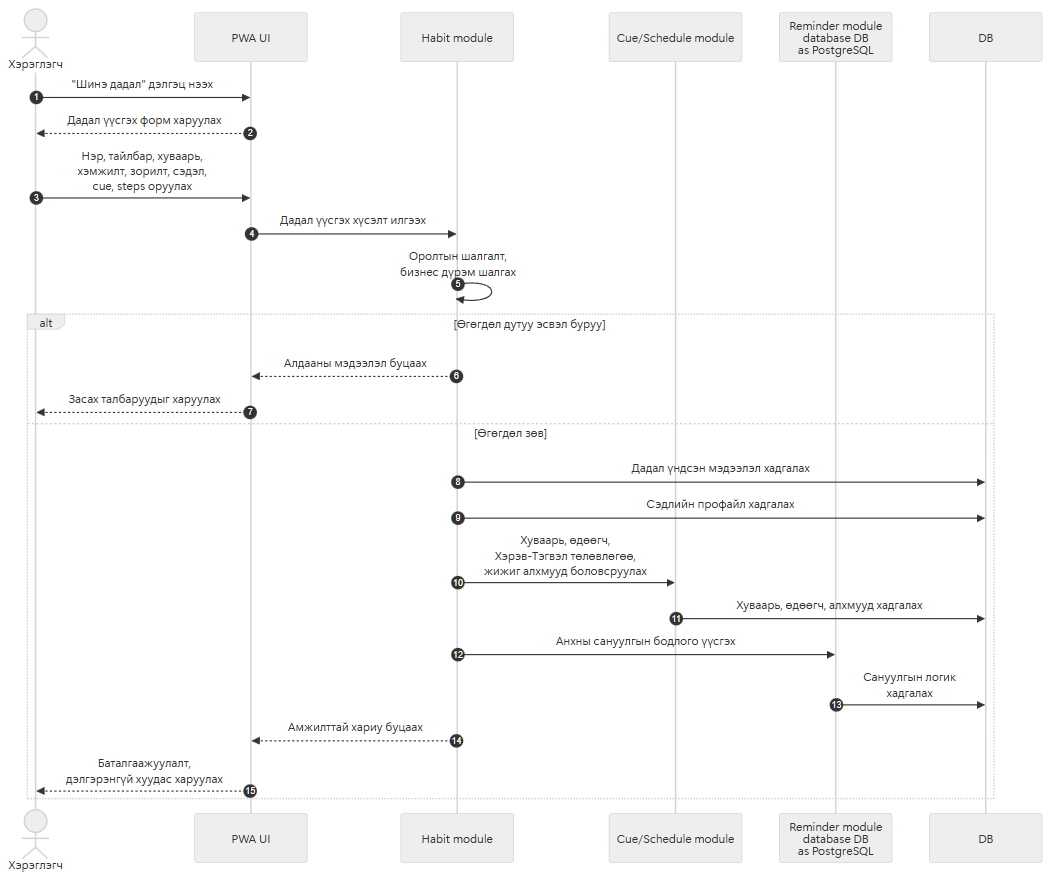
\includegraphics[width=\textwidth,height=0.82\textheight,keepaspectratio]{images/SequenceDiagram1.png}
    \caption{Дадал үүсгэх ба тохируулах дарааллын диаграмм}
\end{figure}

\begin{figure}[H]
    \centering
    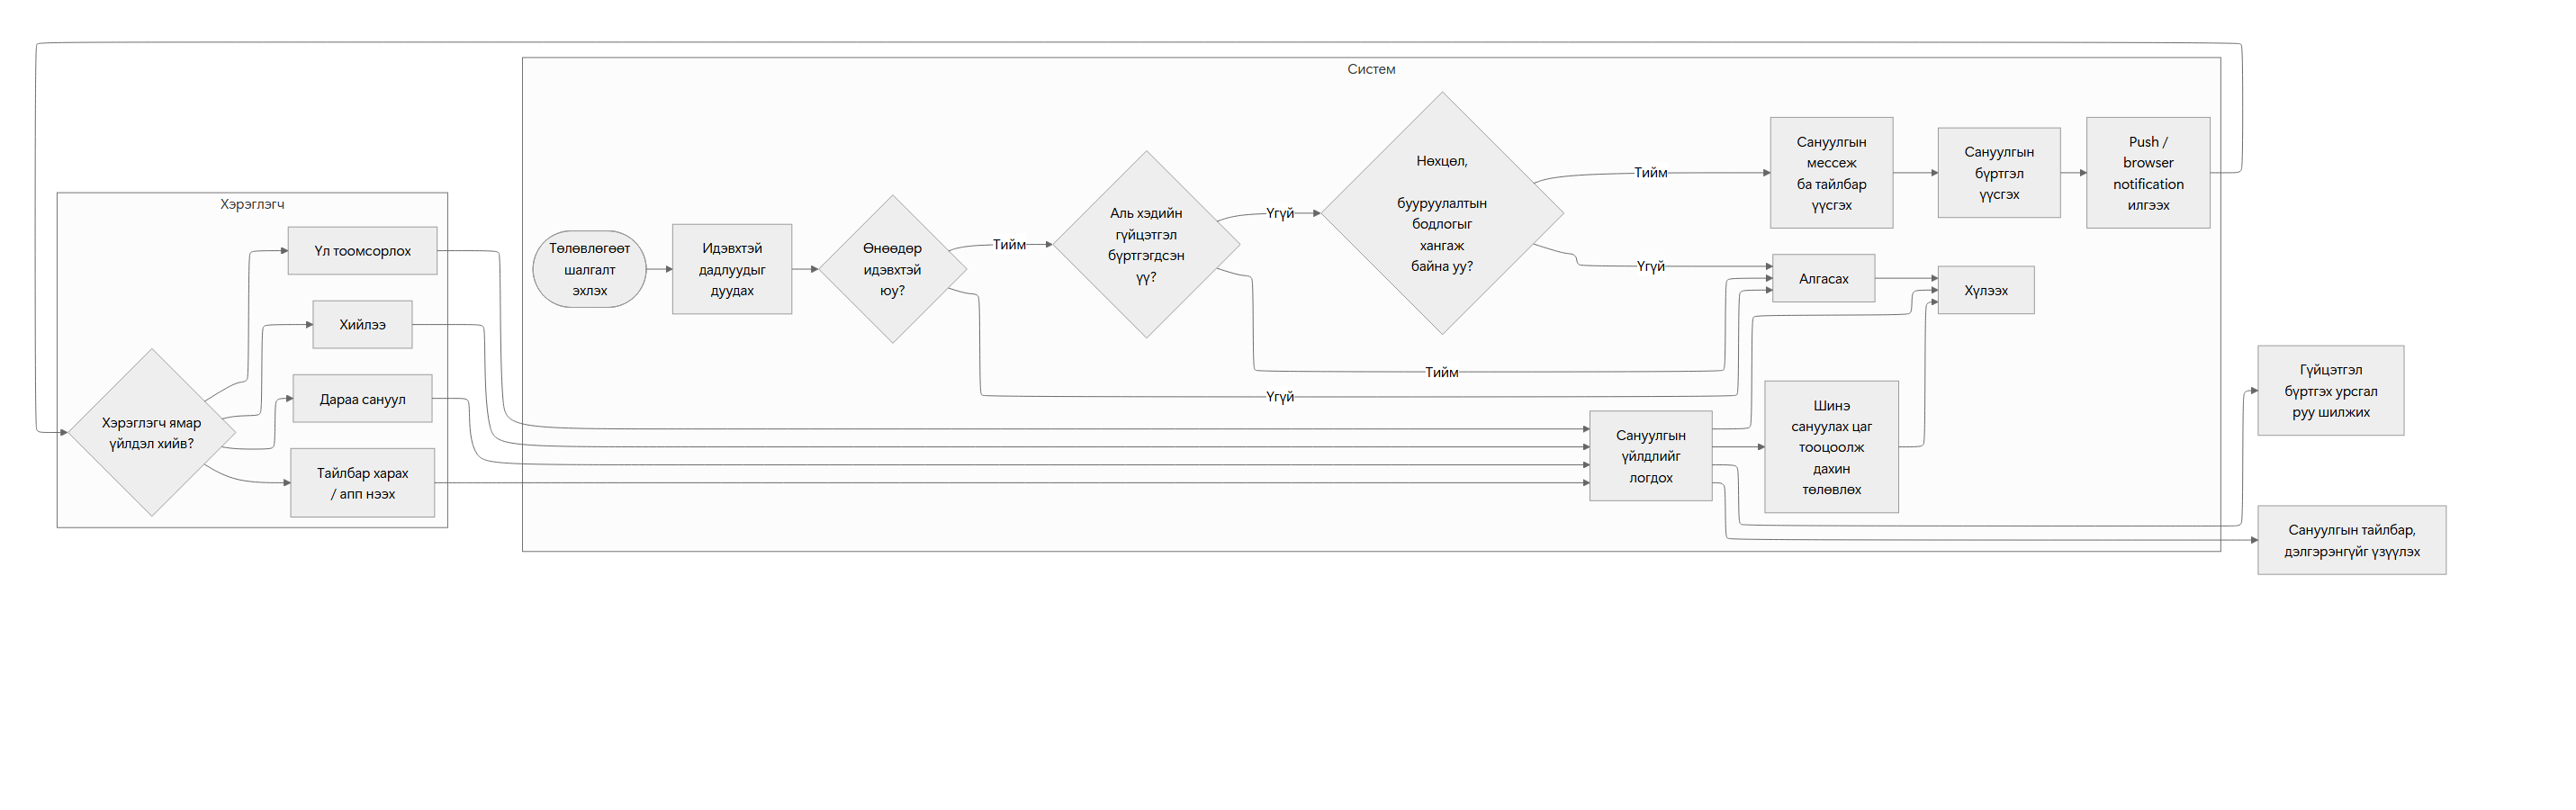
\includegraphics[width=\textwidth,height=0.82\textheight,keepaspectratio]{images/ActivityDiagram3.png}
    \caption{Нөхцөл байдалд суурилсан сануулга шийдвэрлэх ба хүргэх үйл ажиллагааны диаграмм}
\end{figure}

\begin{figure}[H]
    \centering
    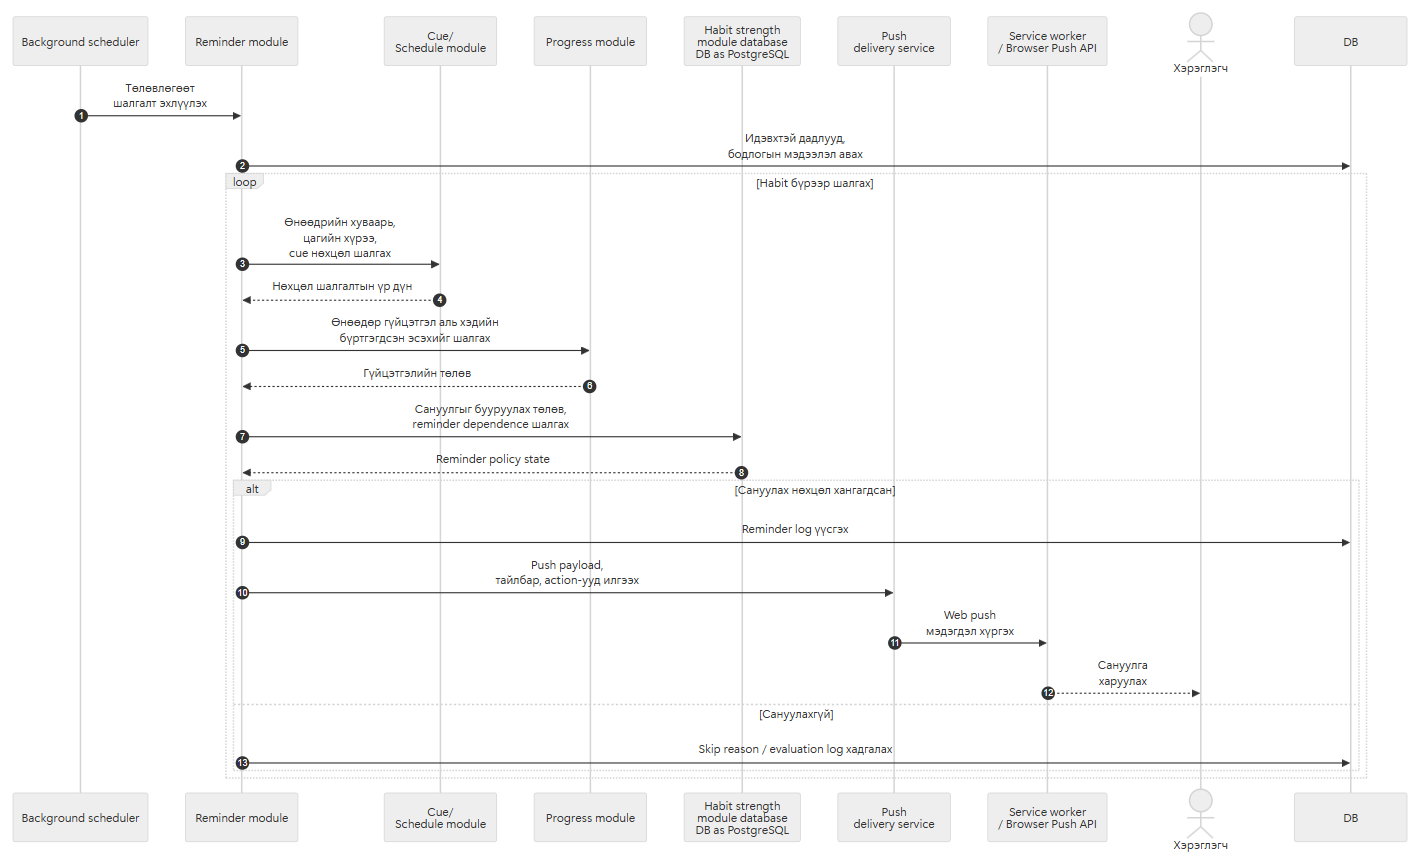
\includegraphics[width=\textwidth,height=0.82\textheight,keepaspectratio]{images/SequenceDiagram2.png}
    \caption{Нөхцөл байдалд суурилсан сануулга шийдвэрлэх ба хүргэх дарааллын диаграмм}
\end{figure}

\begin{figure}[H]
    \centering
    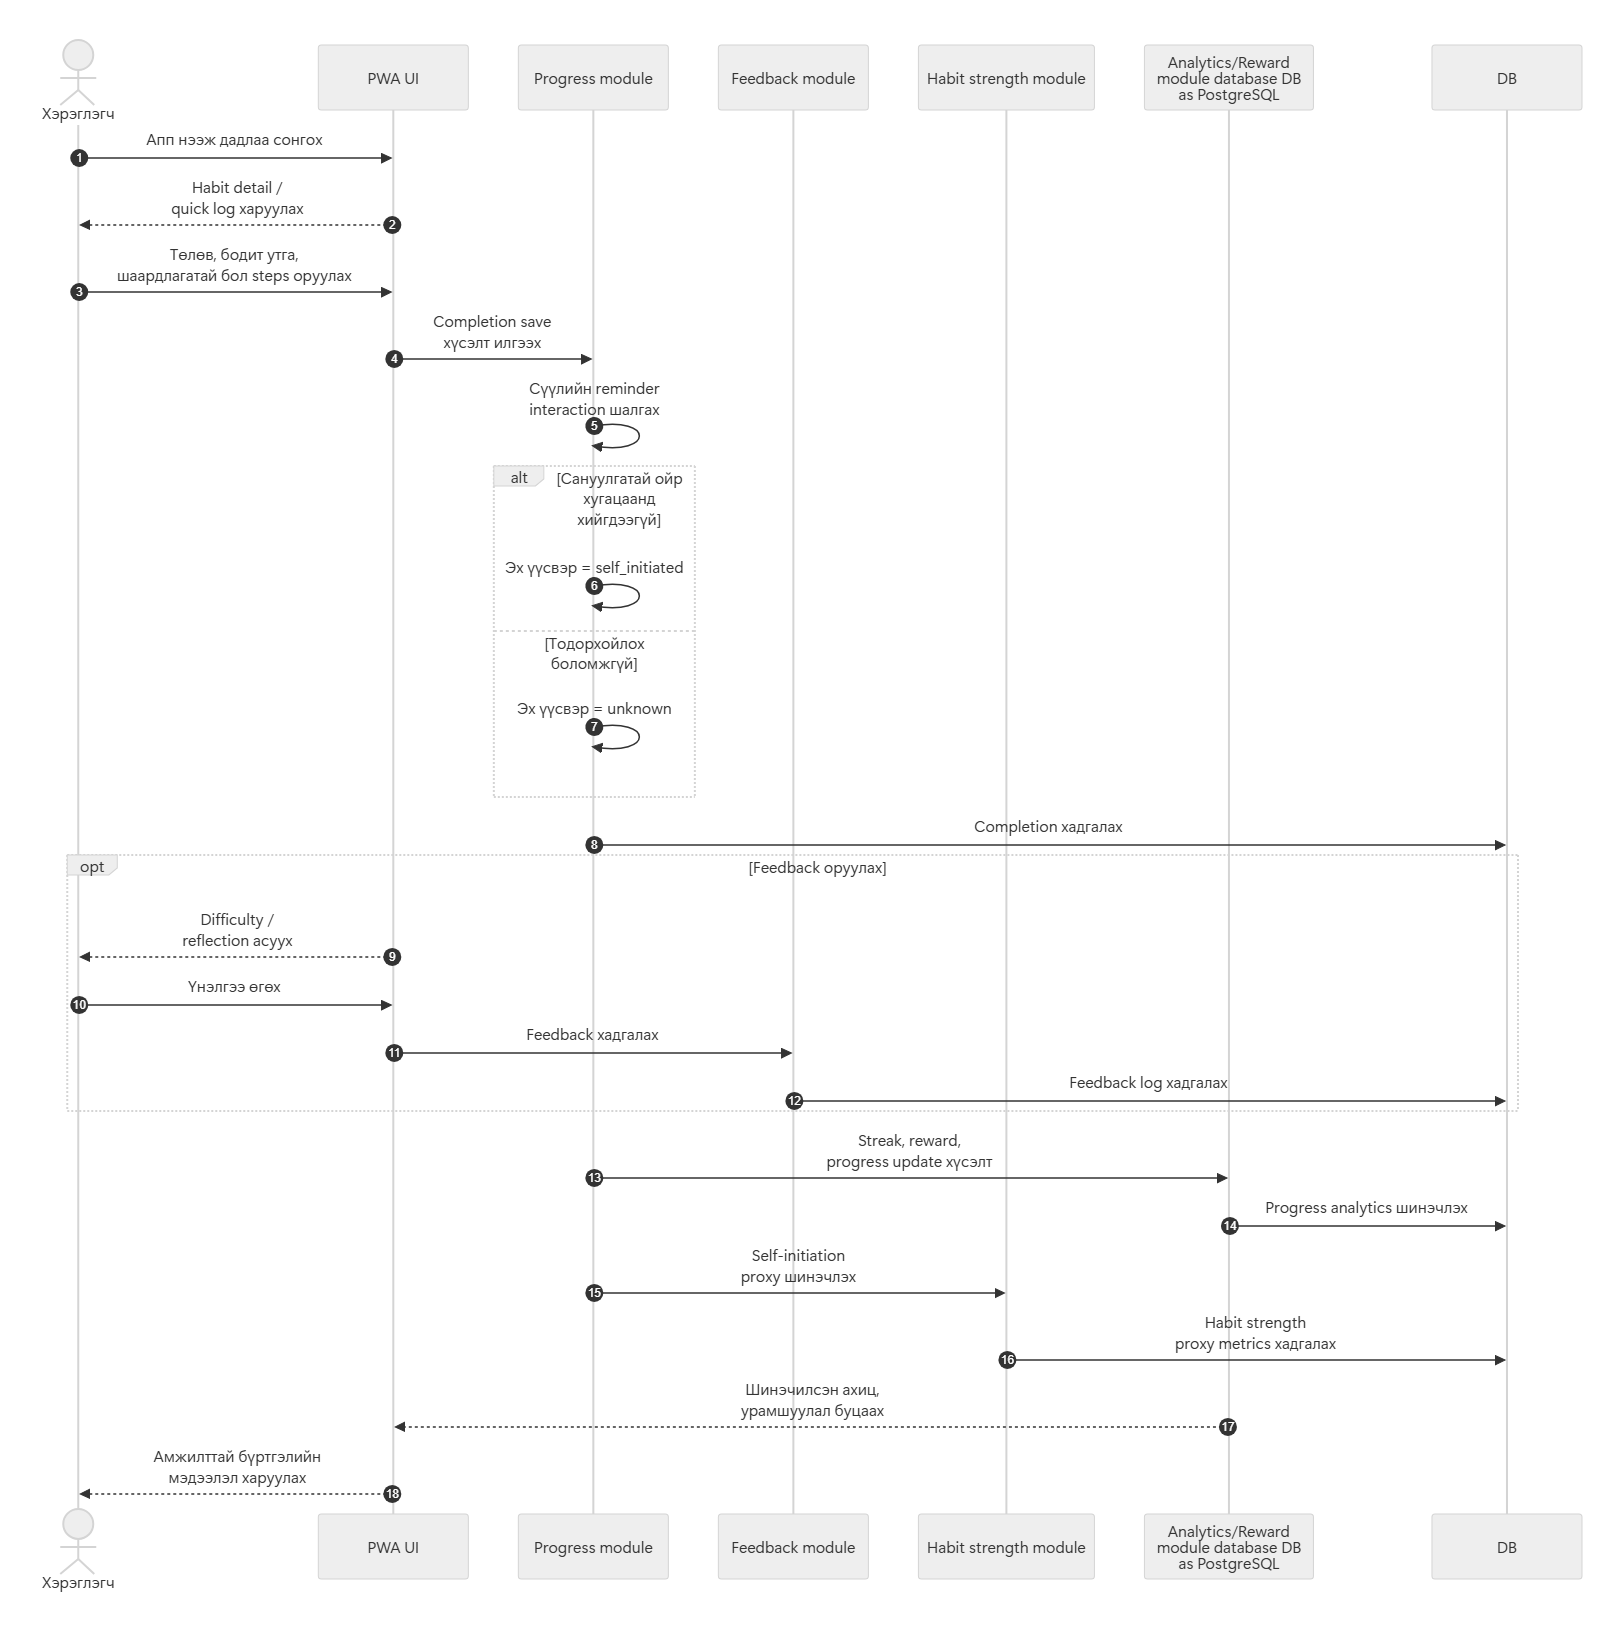
\includegraphics[width=\textwidth,height=0.82\textheight,keepaspectratio]{images/SequenceDiagram4.png}
    \caption{Сануулгагүйгээр өөрийн санаачилгатай гүйцэтгэл бүртгэх дарааллын диаграмм}
\end{figure}

\begin{figure}[H]
    \centering
    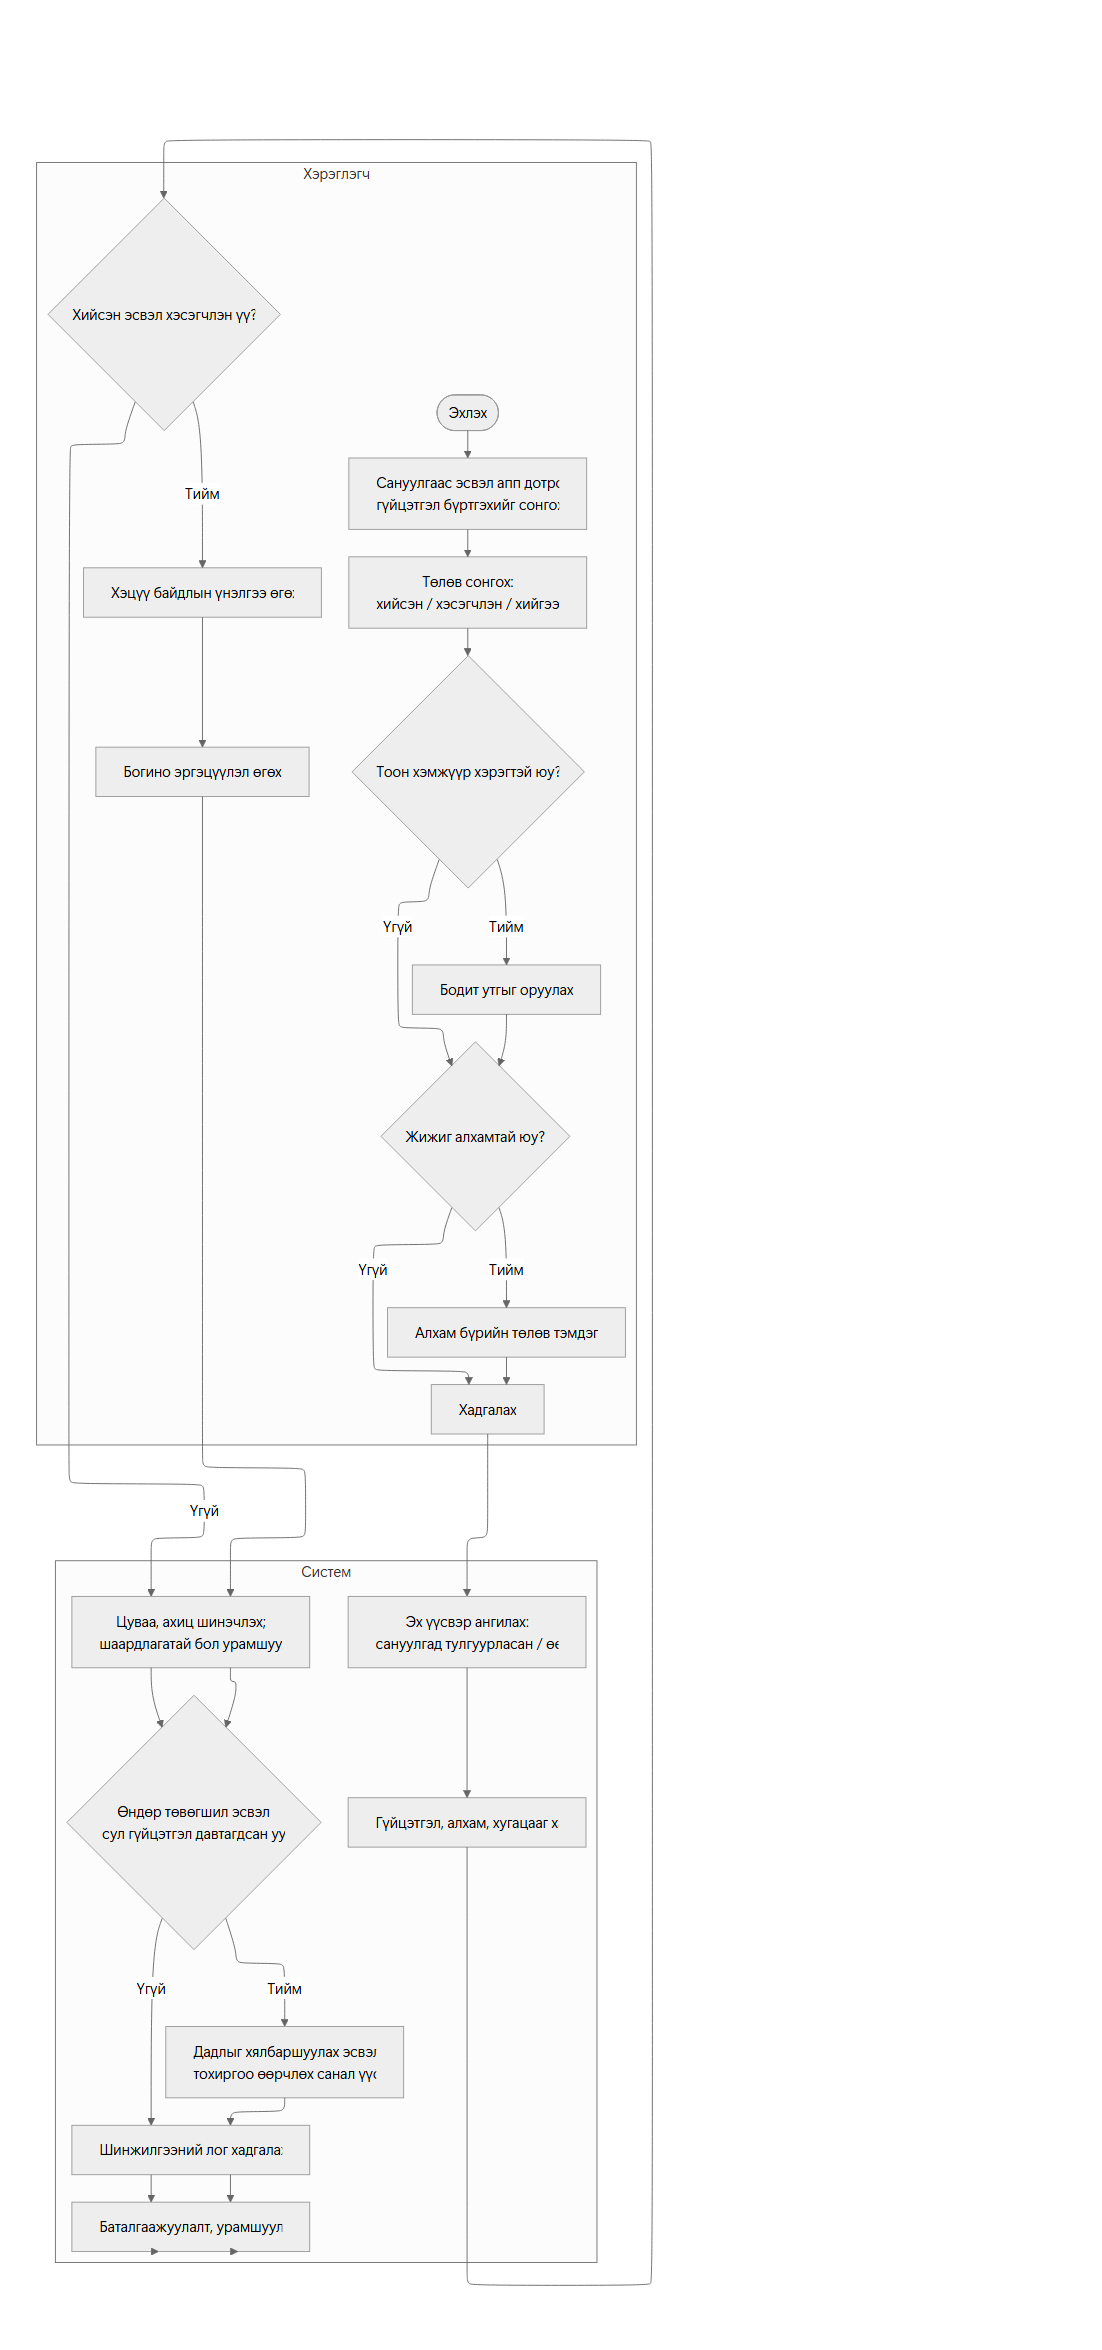
\includegraphics[width=\textwidth,height=0.82\textheight,keepaspectratio]{images/activityDiagram4.png}
    \caption{Гүйцэтгэл бүртгэх, санал сэтгэгдэл авах, урамшуулал идэвхжүүлэх үйл ажиллагааны диаграмм}
\end{figure}

\begin{figure}[H]
    \centering
    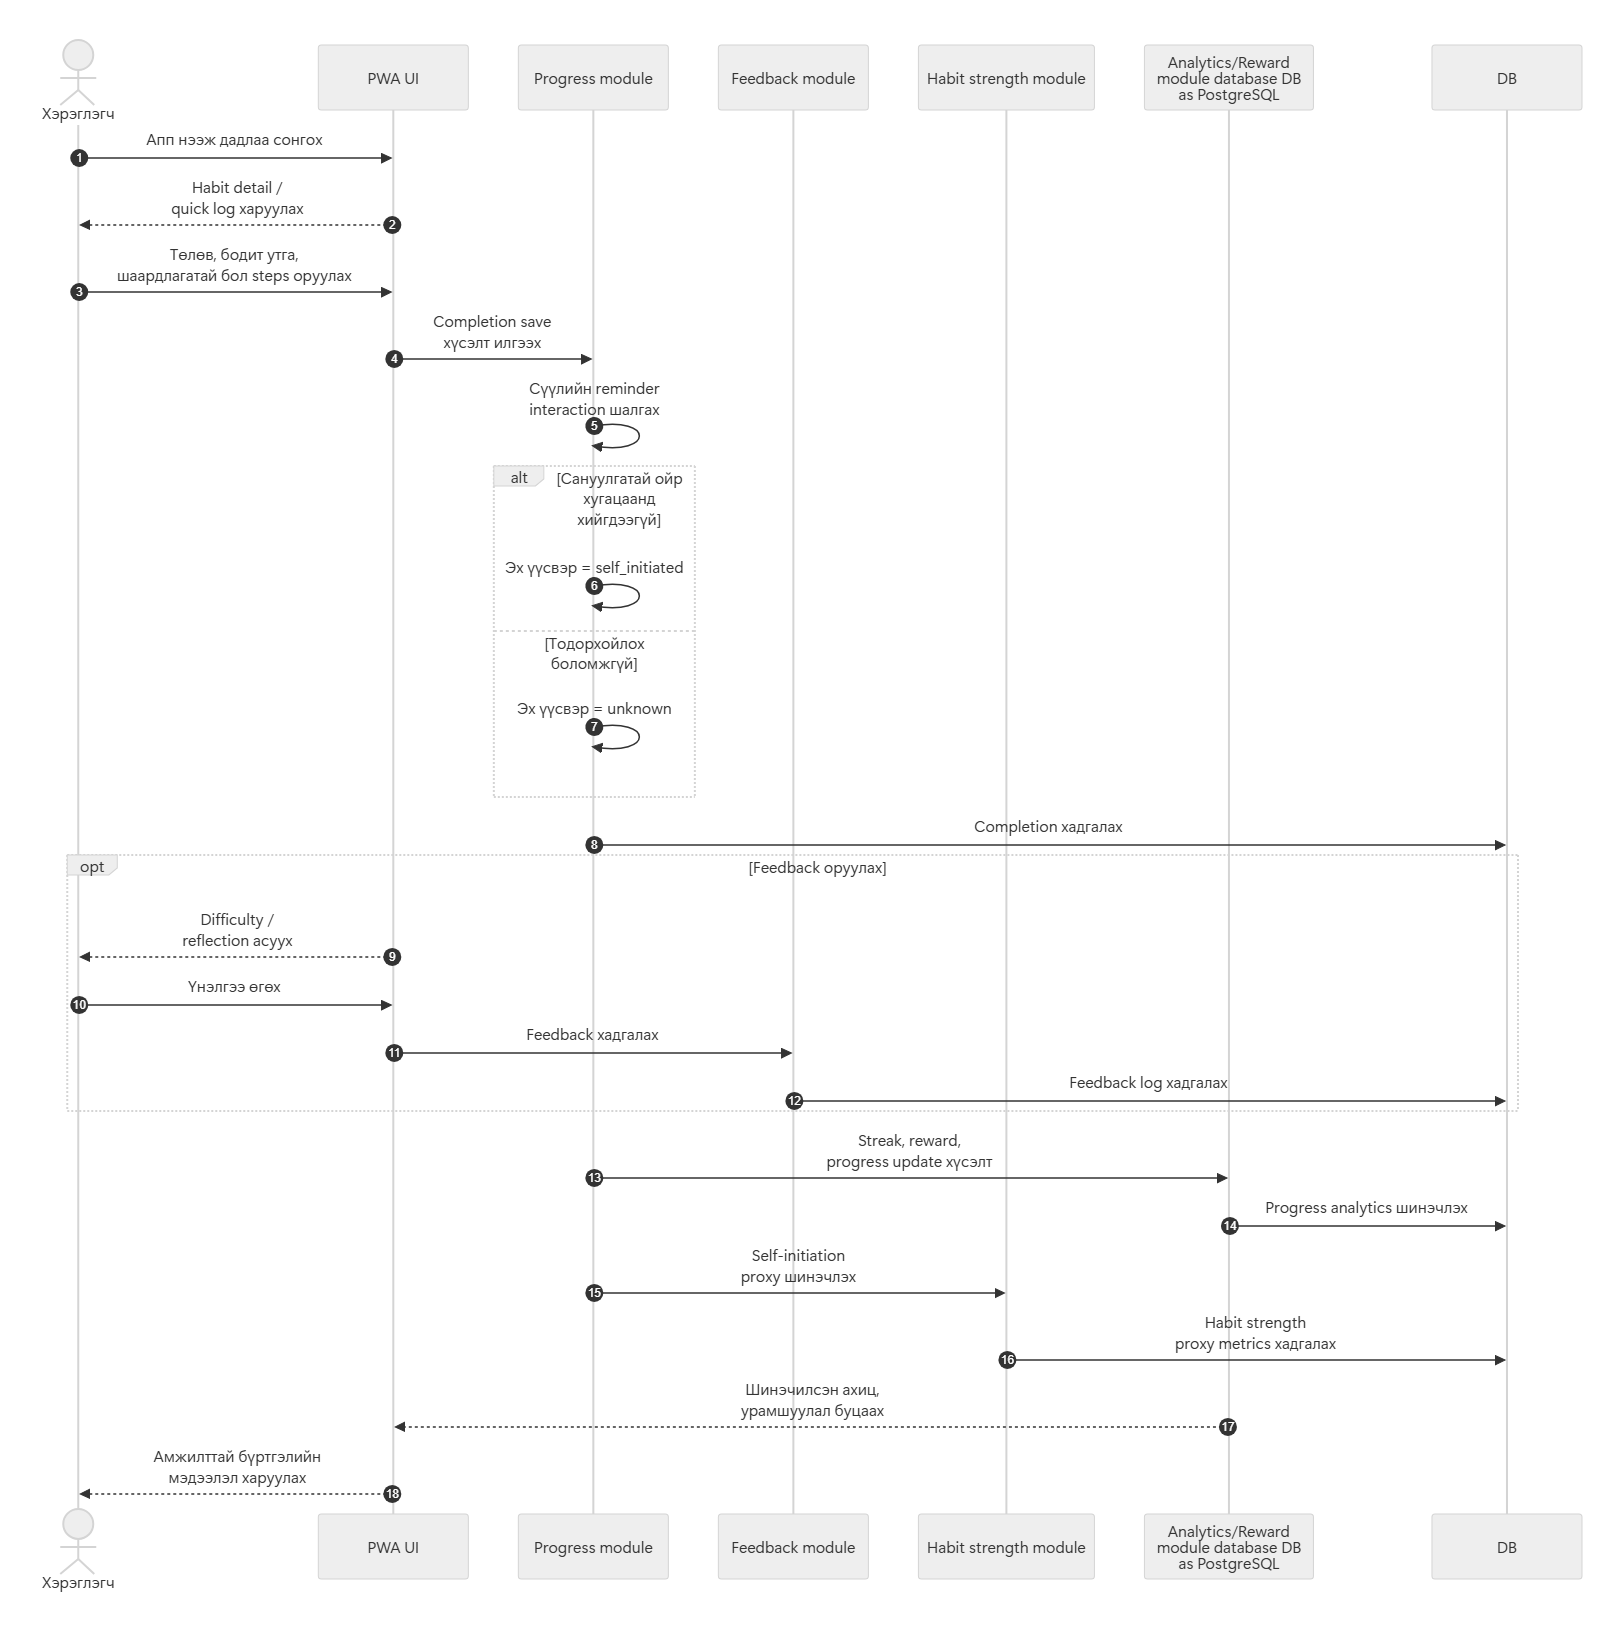
\includegraphics[width=\textwidth,height=0.82\textheight,keepaspectratio]{images/SequenceDiagram3.png}
    \caption{Сануулгад хариулах ба гүйцэтгэл бүртгэх дарааллын диаграмм}
\end{figure}

\begin{figure}[H]
    \centering
    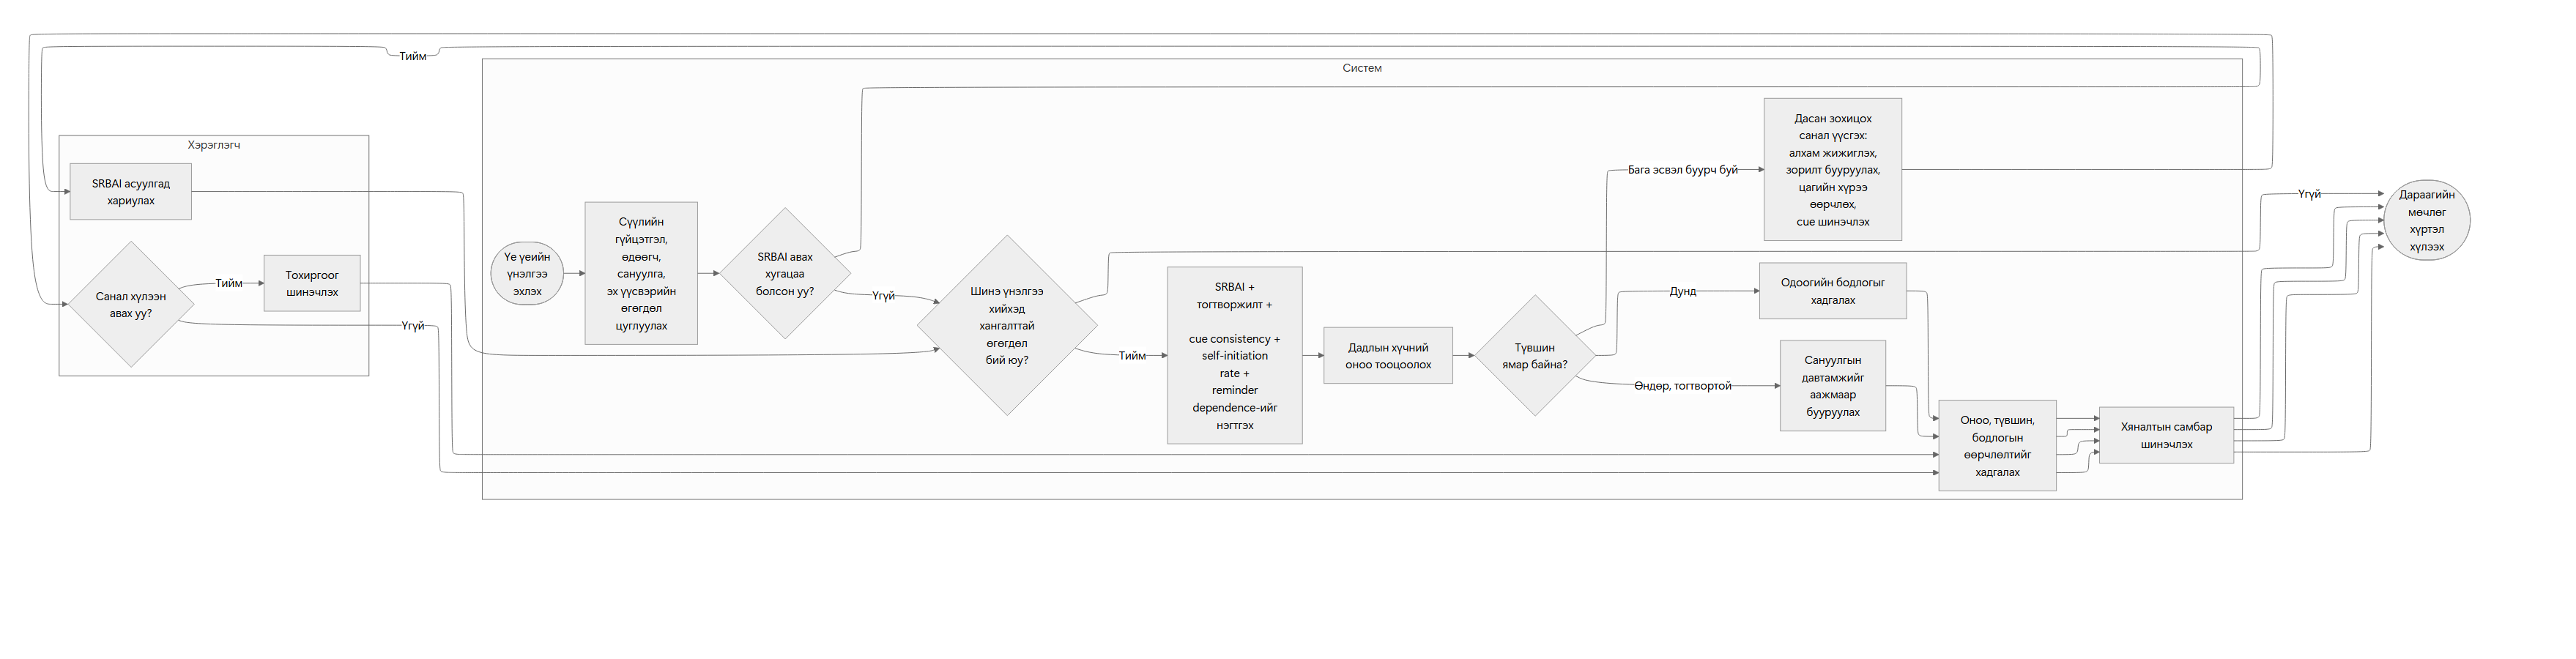
\includegraphics[width=\textwidth,height=0.82\textheight,keepaspectratio]{images/ActivityDiagram5.png}
    \caption{Дадлын хүчний үнэлгээ, сануулгын бодлого шинэчлэх ба дасан зохицох үйл ажиллагааны диаграмм}
\end{figure}

\begin{figure}[H]
    \centering
    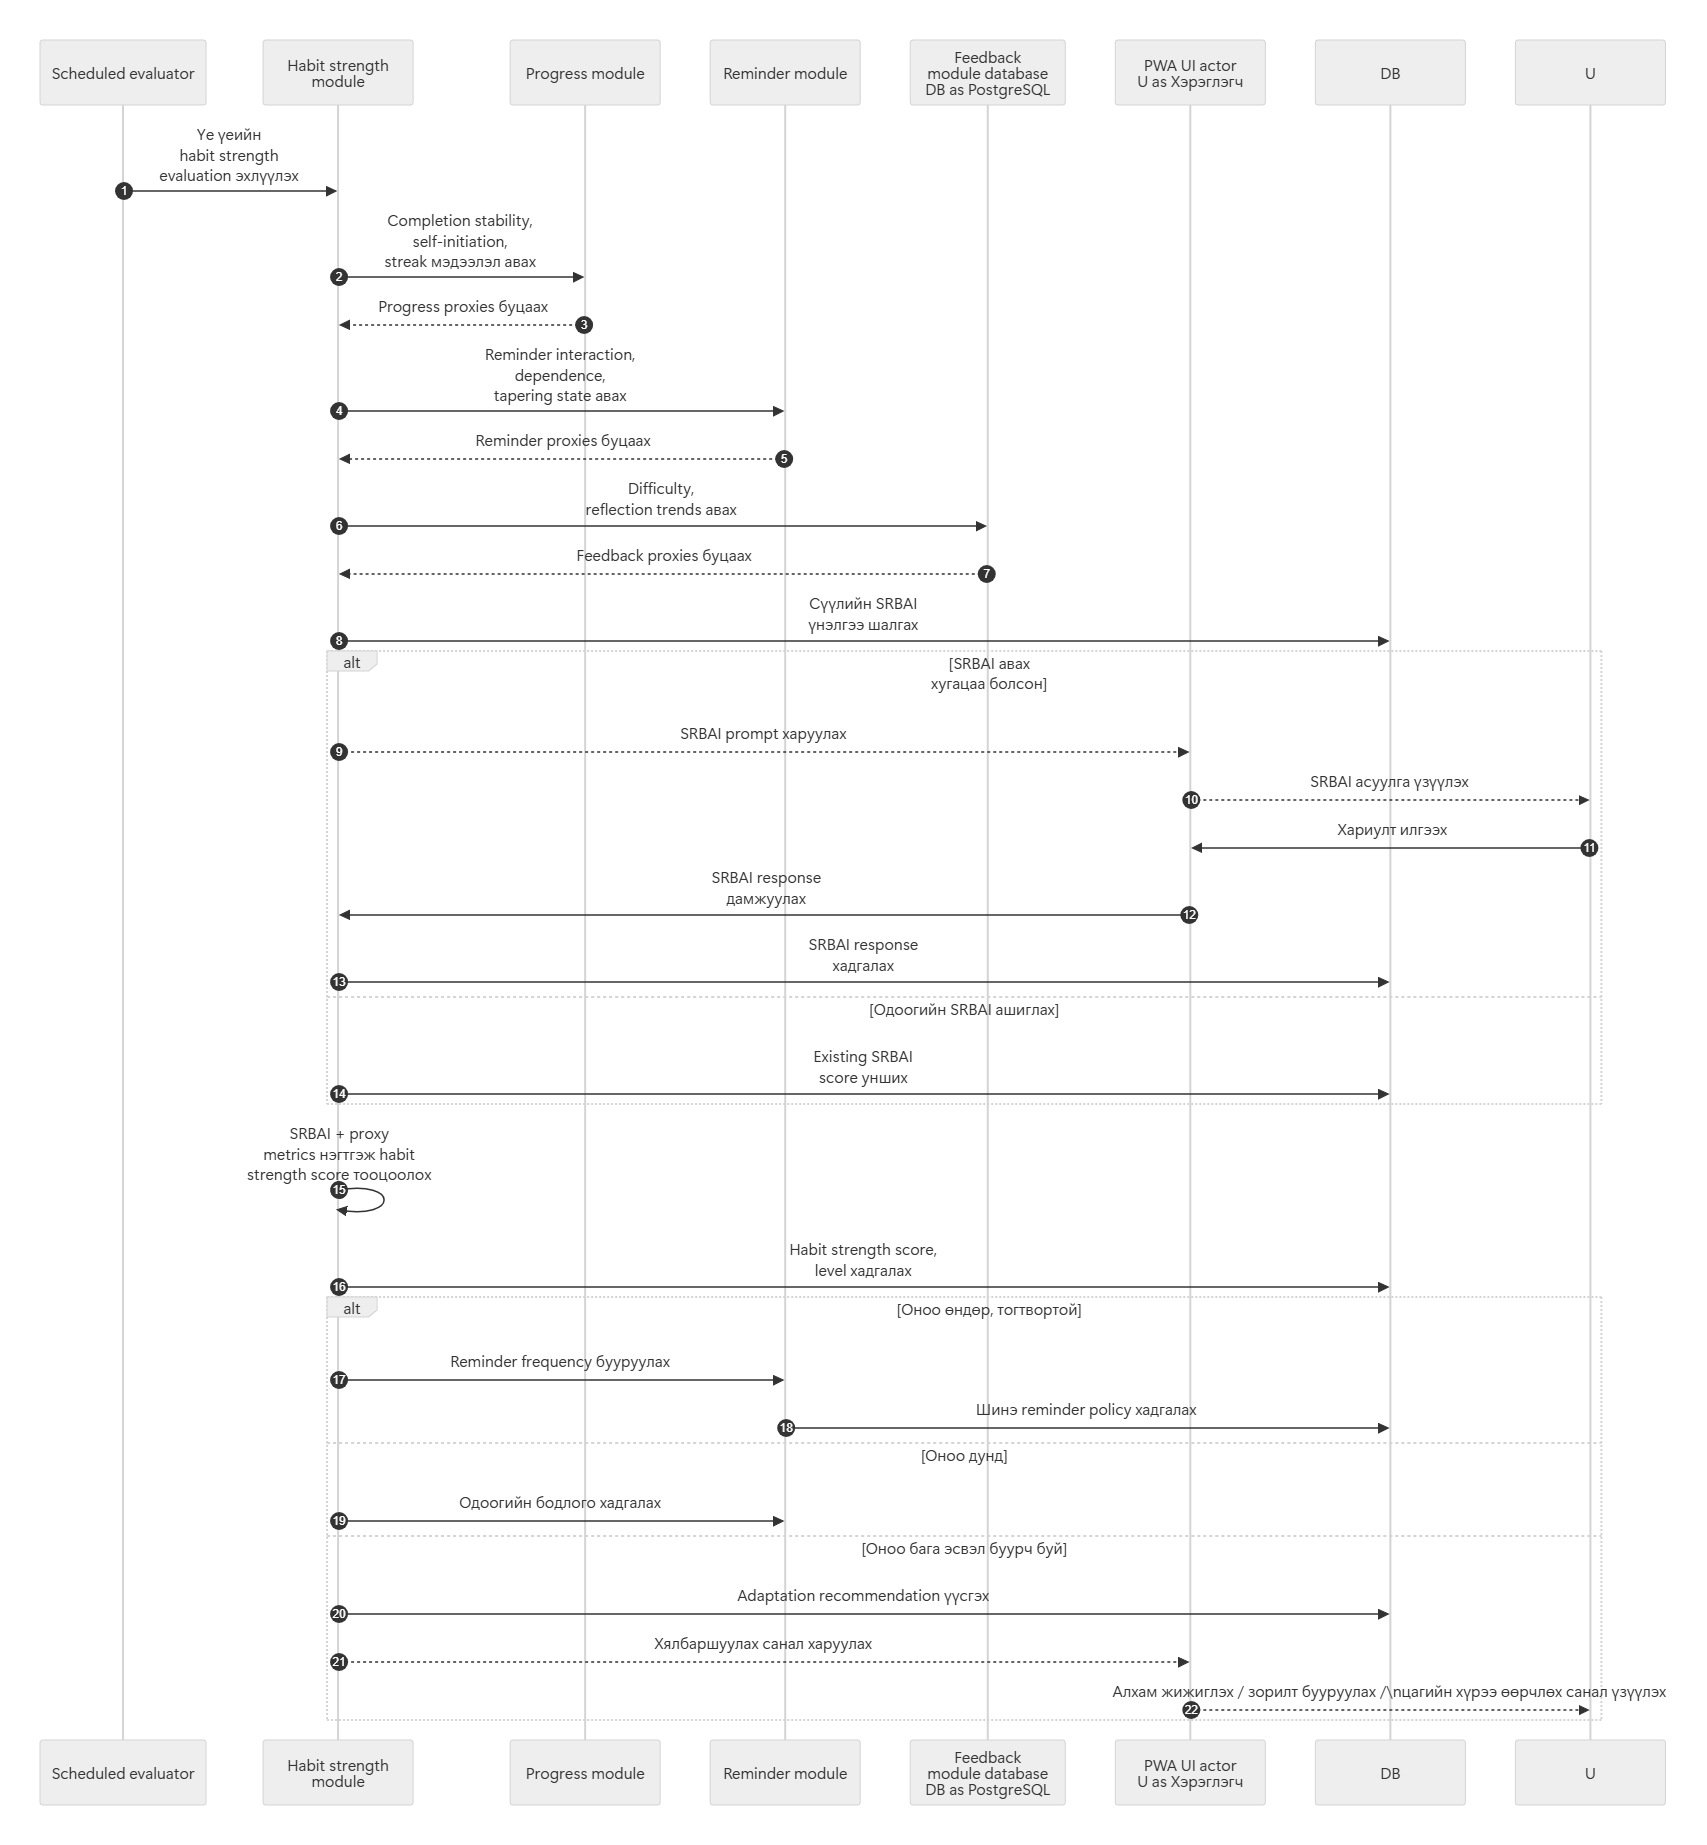
\includegraphics[width=\textwidth,height=0.82\textheight,keepaspectratio]{images/SequenceDiagram5.png}
    \caption{SRBAI үнэлгээ, дадлын хүч тооцоолох ба дасан зохицох дарааллын диаграмм}
\end{figure}

\section{Туршилтын дэлгэрэнгүй хэмжигдэх үзүүлэлтүүд}

\begin{table}[htbp]
\centering
\small
\setlength{\tabcolsep}{4pt}
\begin{tabular}{|L{4.0cm}|L{8.8cm}|}
\hline
\textbf{Үзүүлэлтийн бүлэг} & \textbf{Хэмжигдэх үндсэн үзүүлэлтүүд} \\
\hline
Өдөөгч дохио ба сануулга & Өдөөгч нөхцөл тохируулсан хувь, сануулга нээсэн хувь, сануулгад үйлдэл сонгосон хувь, сануулгын үйлдлийн тархалт, сануулгын цаг тохиромжтой байсан хувь, сануулгын давтамжийн өөрчлөлт \\
\hline
Сэдэл ба эргэцүүлэл & Сэдлийн профайл бүрдүүлсэн хувь, ашиг тусын мэдээлэл үзсэн хувь, эргэцүүлэл бөглөсөн хувь, зорилготой нийцэж буй субъектив үнэлгээ \\
\hline
Гүйцэтгэл ба төвөгшил & Нийт гүйцэтгэлийн хувь, хэсэгчлэн гүйцэтгэлийн хувь, гүйцэтгэл бүртгэхэд зарцуулсан хугацаа, жижиг алхмын гүйцэтгэлийн хувь, ``хэрэв--тэгвэл'' төлөвлөгөө үүсгэсэн хувь, хэцүү байдлын оноо, хялбаршуулах санал хүлээн авсан хувь \\
\hline
Тогтворжилт ба дотооджилт & Сануулгагүй нөхцөл дэх гүйцэтгэлийн хувь, тасралтгүй гүйцэтгэлийн цувааны урт, сэргээх боломж ашигласан хувь, автоматжилтын оноо, дадлын хүчний оноо, сануулгаас хэт хараат байдлын үзүүлэлт \\
\hline
Хэрэглээ ба оролцоо & 1, 7, 30 дахь өдрийн эргэн ирэлтийн үзүүлэлт, ахицын өөрчлөлтийн чиг хандлага, хуваалцах үйлдлийн хувь \\
\hline
\end{tabular}
\caption{Хэмжигдэх үндсэн үзүүлэлтүүдийн дэлгэрэнгүй хүснэгт}
\end{table}
